\subsubsection{Elección de microcontrolador}

En los modelos anteriores dentro de la familia de robots Hermes se utilizó distintos sistemas embebidos para su implementación. A continuación se expone una tabla comparativa acerca de las opciones relevadas para esta nueva implementación:

\begin{center}
    \begin{tabular} {
        | >{\centering\arraybackslash}m{3cm}
        | >{\centering\arraybackslash}m{2.25cm}
        | >{\centering\arraybackslash}m{2.25cm}
        | >{\centering\arraybackslash}m{2.25cm} 
        | >{\centering\arraybackslash}m{2.25cm} |}
        \hline \rowcolor{test_header_color}
            Caracteristica & ESP-32 & Arduino Mega 2560 & Raspberry Pi 3 B+ & NVIDIA Jetson TK1\\
        \hline
            Procesador & Xtensa LX6 & ATMEGA 2560 & ARM Cortex A53 & ARM Cortex A15 \\
        \hline
            Frecuencia CPU & 240 MHz & 16 MHz & 1,4 GHz & 2,3 GHz \\
        \hline
            WiFi/Bluetooth & Si & Requiere módulo externo & Si & Requiere módulo externo \\
        \hline
            Periféricos & {Wi-Fi, Bluetooth, ADC, DAC, SPI, I2C, UART, PWM, GPIOs, SD/MMC, contador de pulsos, Timers} & {UART, I2C, SPI, ADC, PWM, GPIOs, Timers, USB} & {Wi-Fi, Bluetooth, Ethernet, HDMI, USB x4, GPIOs, I2C, SPI, UART, PWM} & {USB 3.0/2.0, HDMI, Ethernet, SATA, SD/MMC, PCIe x4, GPIOs, I2C, SPI, UART, PWM, soporte para CUDA} \\
        \hline
            Consumo activo & 160-250 mW & 500 mW & 3,7-5 W & 10-12 W \\
        \hline
            Modo bajo consumo & Si & Si & No & No \\
        \hline
            Sistema Operativo & FreeRTOS & Bare metal & Linux & ROS \\
        \hline
            Costo estimado (USD) & \$10 & \$30 & \$45 & \$150 \\
        \hline
    \end{tabular}
\end{center}

Analizando las principales características de cada placa se puede ver que todas cumplen
parcialmente con los requerimientos de hardware para este proyecto, pero, la que se destaca por su costo, periféricos, conectividad y consumo activo es el microcontrolador ESP-32. 

Para esta nueva edición, además, se planteó la idea de reproducir el robot en varios ejemplares por lo que contar con un sistema embebido de bajo coste resulta una característica principal al momento de elegir un modelo. También se busca una placa que se adecúe más a la Industria 4.0 donde los dispositivos se conectan a Internet y es allí donde mandan reportes o reciben instrucciones. Y por último el consumo no es un tema menor ya que el poder mantenerse activo o funcionar con un esquema de bajo consumo resulta altamente atractivo para cualquier dispositivo móvil como lo es un robot. Es por eso que se optó por la utilización del microcontrolador ESP-32. \cite{kolban2017kolban}

\begin{figure}[H]
   \centering
   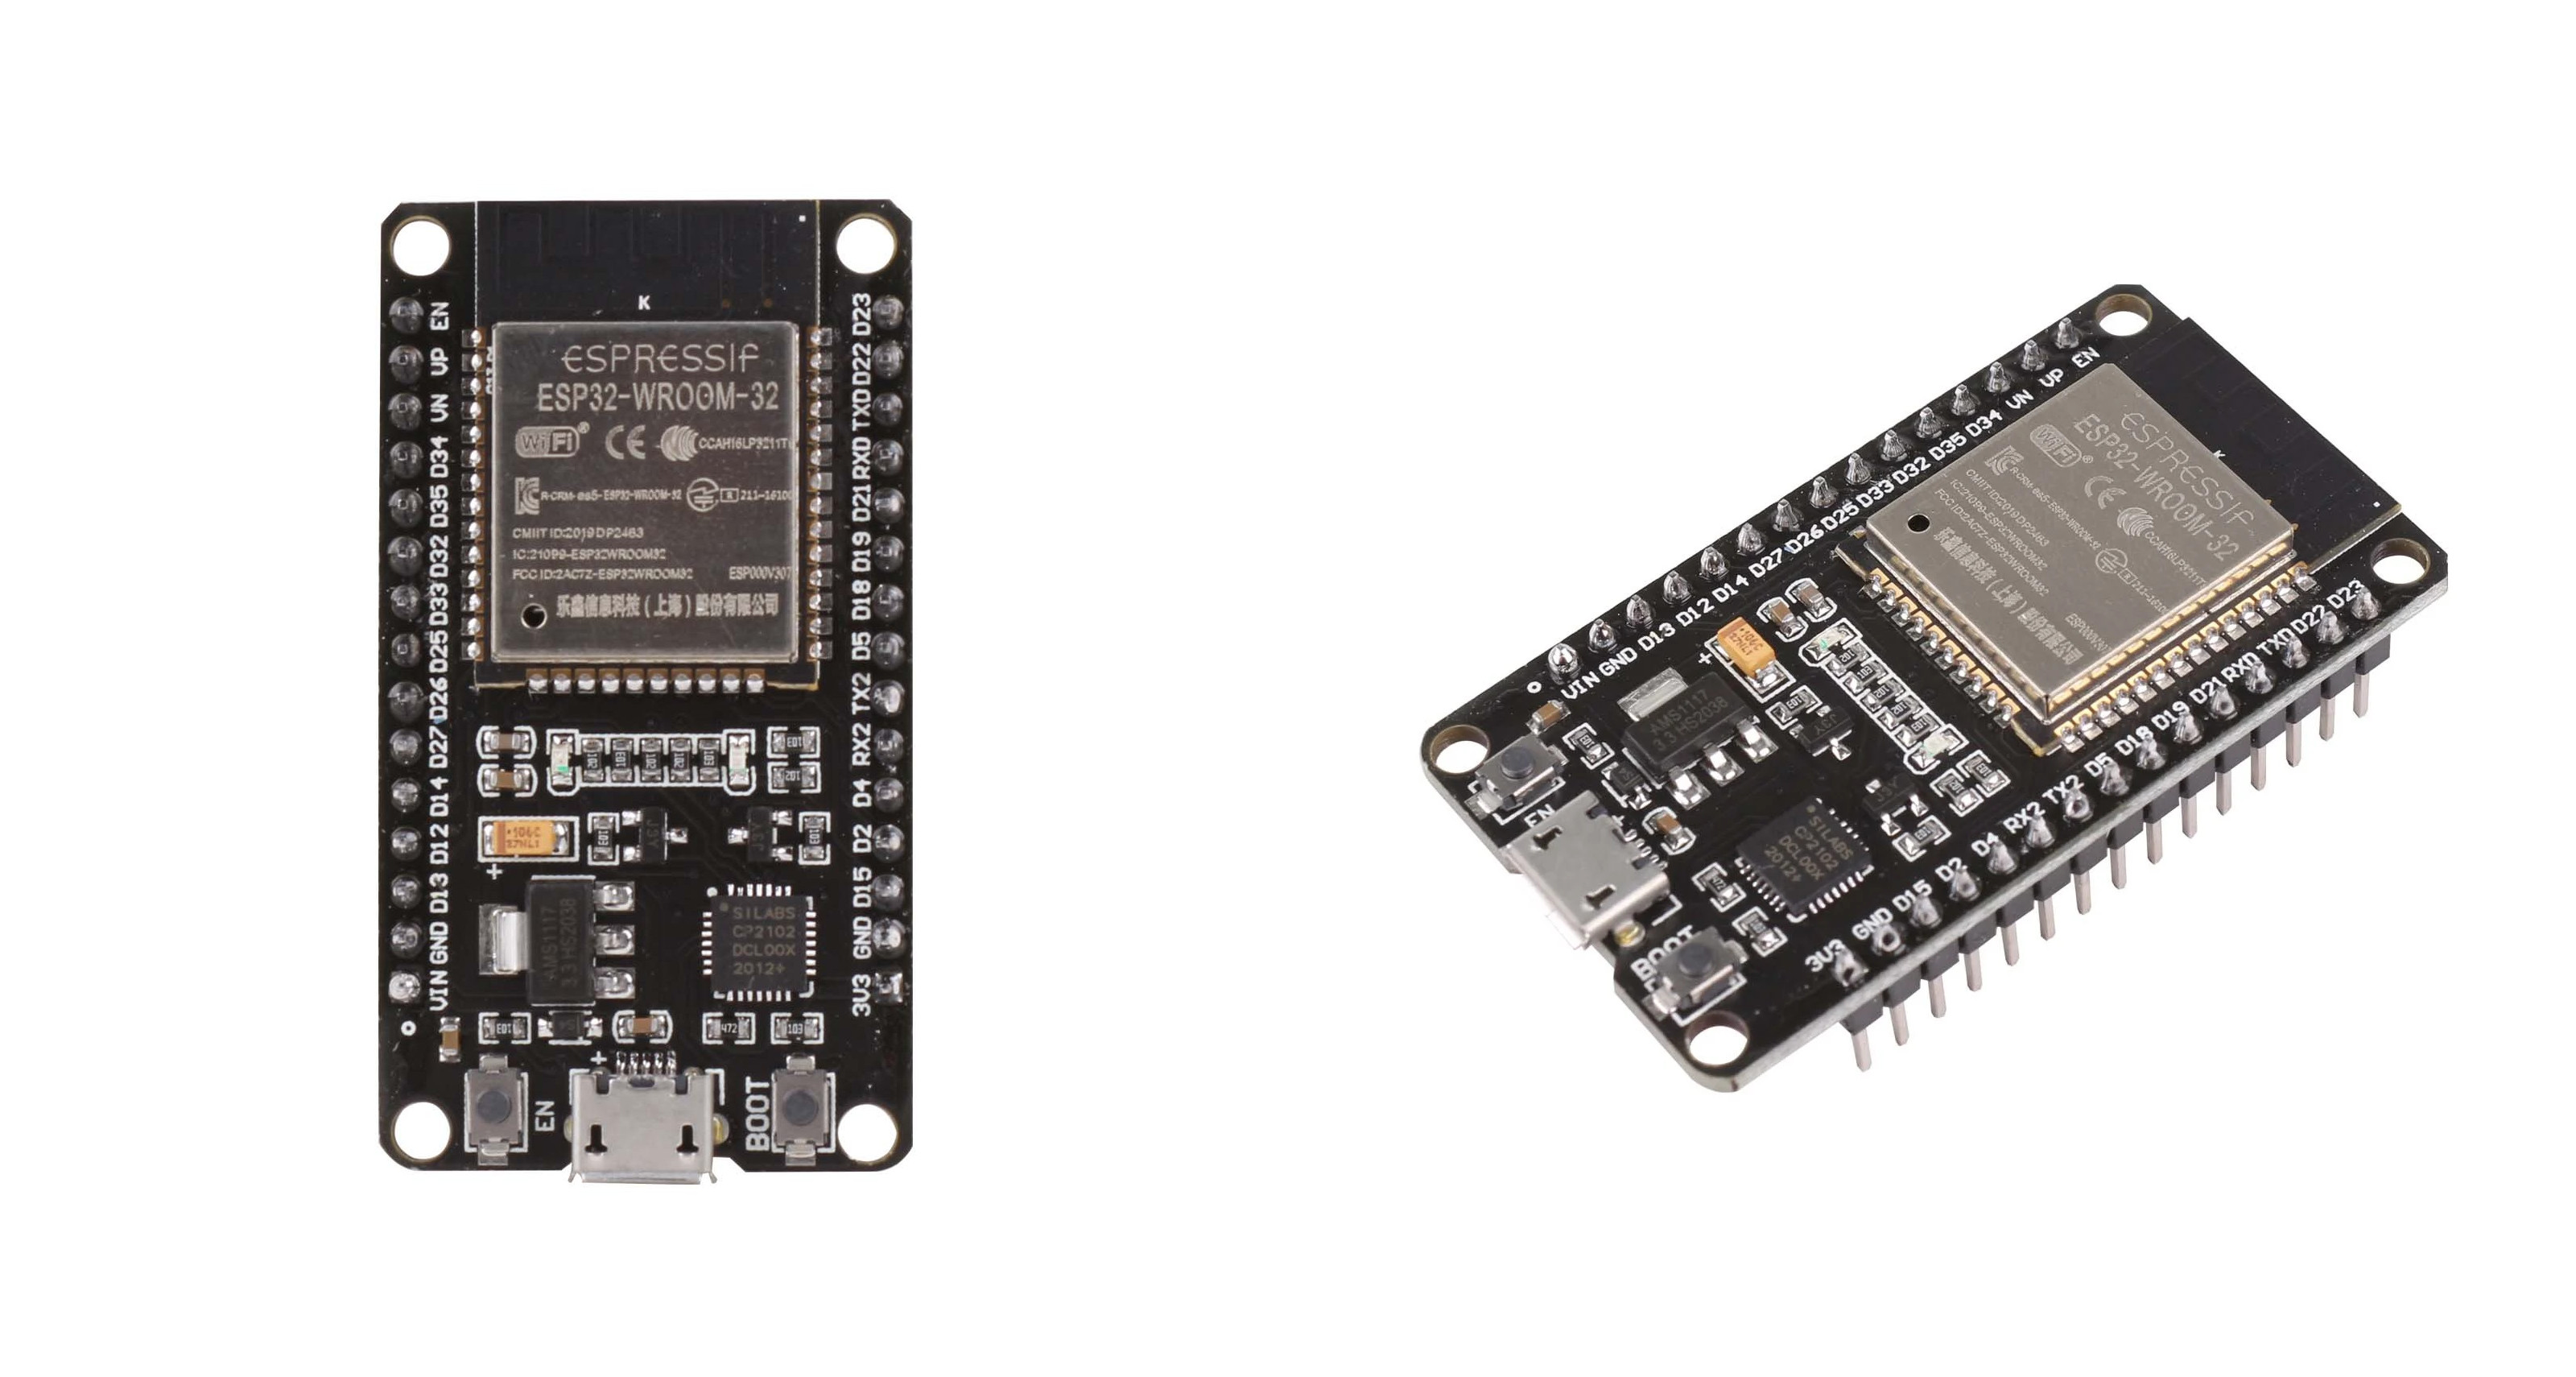
\includegraphics[width=0.7\linewidth]{images/esp32-micro.jpg}
   \caption{Microcontrolador ESP32}
   \label{fig:microcontrolador}
\end{figure}